\section{Agent Framework}  
\label{sec:framework}  

\subsection{Architecture Overview}

\begin{figure*}[ht] 
\centering 
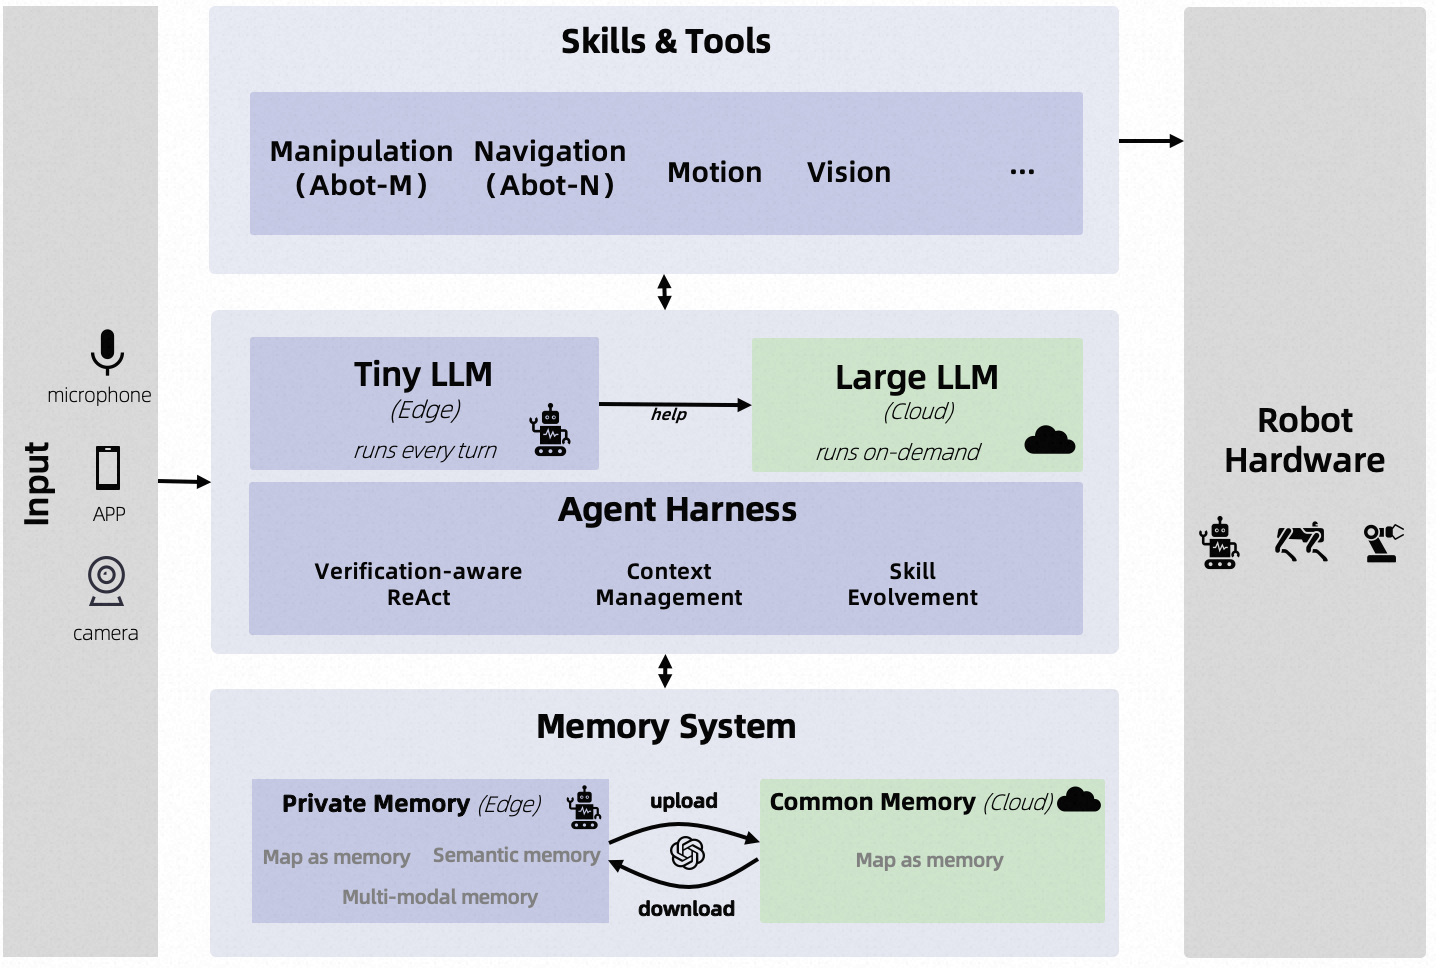
\includegraphics[width=0.7\linewidth]{figure/agentv6.png}
\caption{System architecture of the proposed robot agent. Inputs from multiple sources (microphone, APP, camera) to a dual-LLM core, where a Tiny LLM on the edge handles every turn and escalates to a cloud-based Large LLM on demand. The Agent Harness manages verification-aware ReAct loop, context, and skill evolvement, enabling an extensible skill library (Manipulation, Navigation, Motion, Vision, etc.). A hierarchical Memory System synchronizes private edge memory with shared cloud memory to support cross-robot knowledge transfer. Outputs are dispatched to the robot hardware for execution. } %最终文档中希望显示的图片标题
\label{Fig.main2} %用于文内引用的标签
\end{figure*}


ABot-AgentOS is a general-purpose robotic Agent Operating System
designed for embodied intelligence, providing a deliberative agent layer
above robot hardware and low-level controllers. Rather than replacing existing control stacks, ABot-AgentOS provides a unified cognitive layer that connects multi-modal perception, memory, reasoning, planning, and skill execution across heterogeneous robotic platforms, including humanoids, quadruped robot dogs, mobile manipulators, and robotic arms.

As shown in Figure~\ref{Fig.main2} , ABot-AgentOS receives multi-modal inputs from microphones, mobile applications, cameras, and other sensors, and maps them into a runtime loop for perception, reasoning, and action. The runtime adopts an edge-cloud collaborative LLM architecture. A lightweight Tiny LLM runs on the edge at every interaction turn, enabling low-latency perception, instruction understanding, state tracking, and routine decision-making. When the task requires more complex reasoning, long-horizon planning, or ambiguity resolution, the system can request help from a cloud-based Large LLM, which is invoked on demand to provide stronger semantic understanding and planning capability.

The Agent Harness layer contains three key components: Verification-aware ReAct, Context Management, and Skill Evolvement. It organizes prompts, tools, APIs, and execution protocols into a reliable agent loop. Verification-aware ReAct adds a verifier module on top of ReAct to improve the robustness of the agent system. Context Management selects, compresses, and retrieves relevant information from observations, dialogue history, robot states, and memory. Skill Evolvement enables the agent to refine, reuse, and expand its skill set through continuous interaction with the physical world.

% Above the runtime, ABot-AgentOS abstracts robot capabilities into a unified Skills and Tools layer, including manipulation skills such as Abot-M ~\cite{yang2026abot}, navigation skills such as Abot-N ~\cite{chu2026abot},
Above the runtime, ABot-AgentOS abstracts robot capabilities into a unified Skills and Tools layer, including manipulation skills~\cite{yang2026abot}, navigation skills~\cite{chu2026abot,yang2026asyncshieldplugandplayedgeadapter,yang2025cenavflowguidedreinforcementrefinement},
motion control, vision, and other extensible tools. This abstraction allows the same agent system to operate across different robot embodiments while reusing high-level reasoning and task-planning logic.

A central component of ABot-AgentOS is its multi-modal memory system, which consists of edge-side private memory and cloud-side common memory. Private memory stores robot-specific information such as maps, semantic knowledge, multi-modal interaction history, user preferences, and local environmental experiences, enabling personalization and privacy-preserving operation. Common memory aggregates shareable knowledge, such as reusable map representations and general task experiences, and supports upload/download mechanisms for knowledge transfer across robots. In this way, individual robots can learn from their own embodied experiences while benefiting from collective knowledge accumulated by other agents.

Overall, ABot-AgentOS integrates edge intelligence, cloud reasoning, multi-modal memory, and modular skill execution into a unified operating system for general robotic agents. By decoupling high-level cognition from specific hardware embodiments, it provides a scalable foundation for building embodied agents that can perceive, remember, reason, act, and continuously evolve in real-world environments.



\subsection{Agent Harness}


\begin{figure*}[ht] 
\centering 
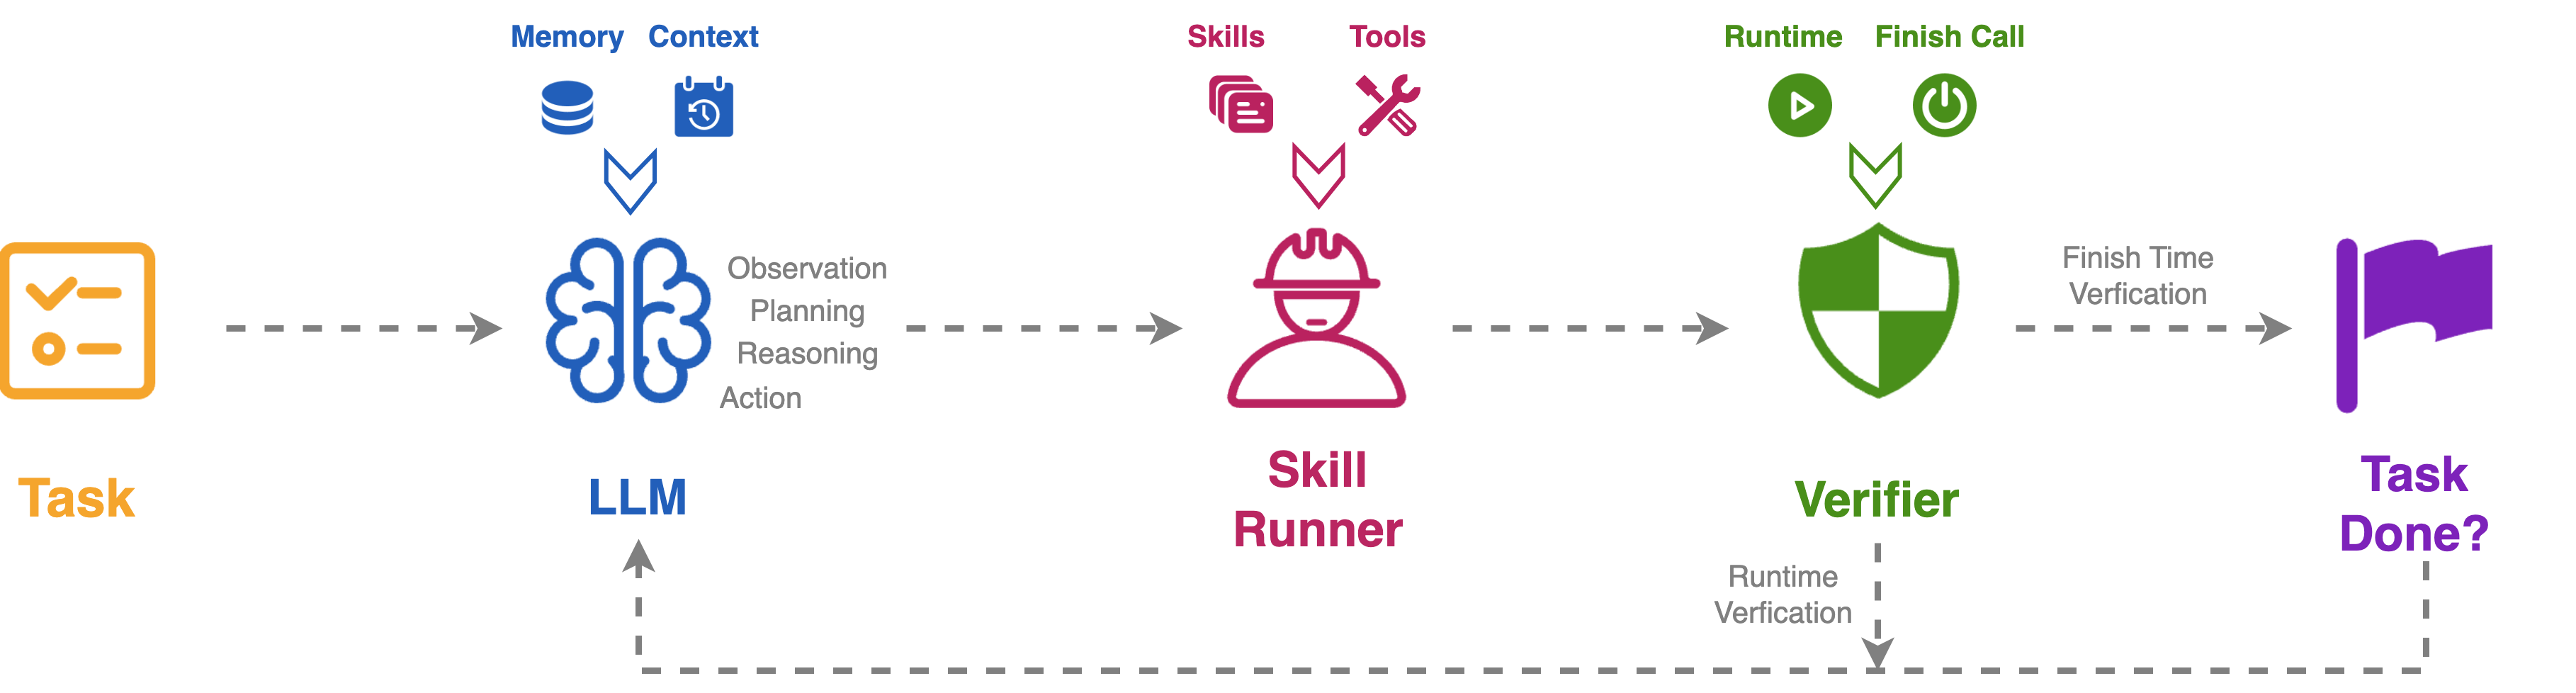
\includegraphics[width=0.98\linewidth]{figure/enhanced_v2_agent_method.drawio.png}
\caption{Overview of the Agent Harness. The main LLM performs scene-conditioned planning with memory and context, delegates procedural subtasks to the Skill Runner, and receives corrective feedback from the Verifier to form a reasoning-execution-verification loop.}
\label{fig:agentworkflow} 
\end{figure*}

% \subsubsection{Overview}

We propose a hierarchical LLM agent framework for long-horizon embodied tasks. The central motivation is that an embodied agent must not only interpret a natural-language instruction, but also understand the scene in which the instruction is grounded, the current execution stage, and the conditions under which the task can be considered complete. Unlike code agents and ordinary tool-use agents, such as SWE-agent for software engineering through agent-computer interfaces~\cite{yang2024sweagent}, Toolformer for API-based tool use~\cite{schick2023toolformer}, and ReAct for interleaved reasoning and acting~\cite{yao2022react}, embodied agents often lack explicit completion signals for intermediate steps. An agent may invoke a navigation command without actually leaving its current location, or rotate and collide repeatedly while still believing, at the language level, that the task is progressing. Our framework therefore does not simply make the LLM call more tools. Instead, it organizes embodied execution as a closed loop of reasoning, execution, and verification.

The framework separates three roles that are often entangled in a single
controller: the main LLM, the Skill Runner, and the Verifier.
As shown in Figure~\ref{fig:agentworkflow}, the task is first processed by a main LLM. Supported by memory and context, the main LLM observes the task, interprets it with respect to the current scene, and forms a high-level plan. It then decides whether to directly invoke a tool or delegate a multi-step subtask to the Skill Runner. The Skill Runner is a skill-level subagent that manages procedural execution in an isolated local context, maintains intermediate state, handles repeated observations and actions, and returns a compressed outcome to the main LLM. The Verifier supervises execution both during runtime and at finish time, checking whether the behavior is still making progress, whether a skill has become stagnant, and whether the task is truly ready to terminate. This loop grounds LLM reasoning in environment facts and reduces procedural drift and premature termination in long-horizon embodied tasks.


\subsubsection{Scene-Conditioned Task Planning}

The main LLM operates as the semantic planner in the Agent Harness. Its
role is to interpret the user instruction with respect to the current
scene, map memory, robot state, recent history, and available skills,
rather than to issue every low-level movement. Before acting, it
determines whether the task requires navigation, search, human
interaction, reporting, manipulation, or additional observation, and it
forms a revisable high-level plan with explicit completion conditions.

This planning step is scene-conditioned rather than purely linguistic.
The same instruction may require different execution strategies
depending on the agent's current location, available visual evidence,
known map structure, reachable regions, nearby objects, and interaction
history. The main LLM therefore reasons about what information is
already sufficient, what must be observed or queried, which skills are
feasible in the current state, and what observable conditions would
constitute completion.

The plan is updated as new observations, tool results, skill summaries,
and verifier feedback enter the context. The main LLM decides which goal
should be pursued, when direct tool use is sufficient, when a subtask
should be delegated to the Skill Runner, and when the task may be ready
to finish. By keeping local execution details out of the main reasoning
thread, the agent preserves a coherent global task state while allowing
lower-level skills to handle procedural detail.

\subsubsection{Skill Runner for Procedural Execution}
The Skill Runner handles subtasks that require sustained local
execution. A skill is not treated as a one-shot tool call or a simple
action macro; it is executed by a skill-level subagent with an isolated
local context that includes the subgoal, recent observations, skill
state, failed attempts, and recovery strategy. The main LLM receives
compressed skill progress and outcomes rather than the full sequence of
intermediate actions.

This context isolation is important for long-horizon embodied tasks,
where local execution may involve repeated movement, observation,
relocalization, view adjustment, and recovery. If every local collision,
short-range movement, failed attempt, or visual adjustment were appended
to the main LLM context, the global objective would be obscured by
procedural detail. The Skill Runner absorbs this local complexity while
preserving the information needed by the main LLM for higher-level
stage management.

During execution, the Skill Runner maintains procedural continuity by
checking whether progress is being made, deciding when additional
observation or local recovery is needed, and determining when control
should return to the main LLM. At termination, it returns a compact
semantic summary indicating whether the subgoal was achieved, why it
failed if it did, what scene information was discovered, what recovery
was attempted, and how the main LLM should use the outcome.

\subsubsection{Multi-Stage Verification}
The Verifier addresses the mismatch between language-level belief and
environment-grounded completion. Unlike many digital tasks, where
success can be checked through explicit external signals such as tests,
API responses, or page states, embodied tasks often require consistency
between the agent's declared progress, the execution trajectory, and the
observed scene state. The Verifier therefore supervises execution by
checking whether recent behavior, skill outcomes, and final answers are
supported by environment evidence rather than by the agent's belief
alone.

Verification is applied at three stages. Runtime verification monitors
whether the recent trajectory and skill state indicate effective
progress or reveal stagnation, repeated collisions, local loops, or
behavior inconsistent with the current plan. Skill-level verification
checks whether a delegated subtask has satisfied its semantic objective,
rather than accepting success solely because a tool or subagent returned
normally. Finish-time verification is performed when the main LLM
attempts to terminate the task; it evaluates the original instruction,
current plan, execution history, skill summaries, observations, and any
new requirements introduced during interaction before allowing the task
to finish.

The Verifier is therefore not merely a final evaluator, but a
supervisory signal inside the Agent Harness. By applying verification
before, during, and after delegated execution, ABot-AgentOS can return
missing conditions to the reasoning layer and reduce stagnation,
misjudgment, and premature termination in open-ended embodied tasks.

\subsubsection{Edge-Cloud Collaborative Routing}

In practical deployment, not every task should be handled by a cloud-scale model. Routine requests can often be completed by an on-device small model and local tools, while long-horizon embodied tasks may require stronger scene understanding, planning, skill execution, and verification. ABot-AgentOS therefore uses an edge-cloud collaborative routing layer: the on-device model first observes the task and context, then either handles the request locally or escalates it to a cloud model for more complex reasoning.

This design follows the general motivation of model routing and hierarchical inference, where systems select among models with different capabilities and costs~\cite{chen2023frugalgpt,ong2024routellm,anthropic2026advisortool}. In our setting, the routing policy is learned from training samples and execution feedback rather than fixed rules. It captures which requests can be reliably solved with local tools, which need cloud-level planning, and which require additional observation before routing. This keeps latency and deployment cost under control while preserving cloud-scale capability for tasks that need deeper long-horizon reasoning.

% This design is related to recent work on model routing and hierarchical inference. FrugalGPT and RouteLLM study how to dynamically select among language models with different capabilities and costs, balancing output quality and inference expense~\cite{chen2023frugalgpt,ong2024routellm}. Anthropic's advisor tool provides a pattern closer to agent execution: a faster and lower-cost executor model can consult a stronger advisor model during long-horizon tasks, so that the high-capability model is invoked mainly for strategic guidance~\cite{anthropic2026advisortool}. Our setting shares the same motivation of avoiding unnecessary use of the largest model, but focuses on how an on-device agent learns when to handle a request locally and when to route it to the cloud, especially when tasks involve embodied skills, visual observation, and long-term state tracking.

% The routing decision is not based on manually fixed task rules. We prepare training samples that cover different task types, scene complexities, and execution outcomes, and let the small model summarize and update its own routing skill based on its performance on these samples. This routing skill captures which tasks can be reliably completed by local tools, which tasks require cloud-level planning, and which tasks require additional observation before a routing decision can be made. This idea echoes Toolformer, where a model learns when to use tools, and Voyager, where an agent accumulates and reuses skills over time~\cite{schick2023toolformer,wang2023voyager}, but here the learned skill is used for edge-cloud task routing.

% Through this edge-cloud collaboration mechanism, the system can keep latency and deployment cost under control while preserving cloud-scale model capability for complex embodied tasks. The on-device small model performs fast filtering and local execution, while the cloud model handles tasks that require deep planning, long-horizon skill execution, and multi-stage verification. As the routing skill is updated from training samples and execution feedback, the system gradually learns a more appropriate allocation between efficiency and capability.
% =========================================================
% Additional packages used in this section if not already loaded:
% \usepackage{amsmath}
% \usepackage{booktabs}
% \usepackage{tabularx}
% \usepackage{float}      % for [H]
% \usepackage{placeins}   % for \FloatBarrier
% =========================================================
\begin{figure}[!t]
    \centering
    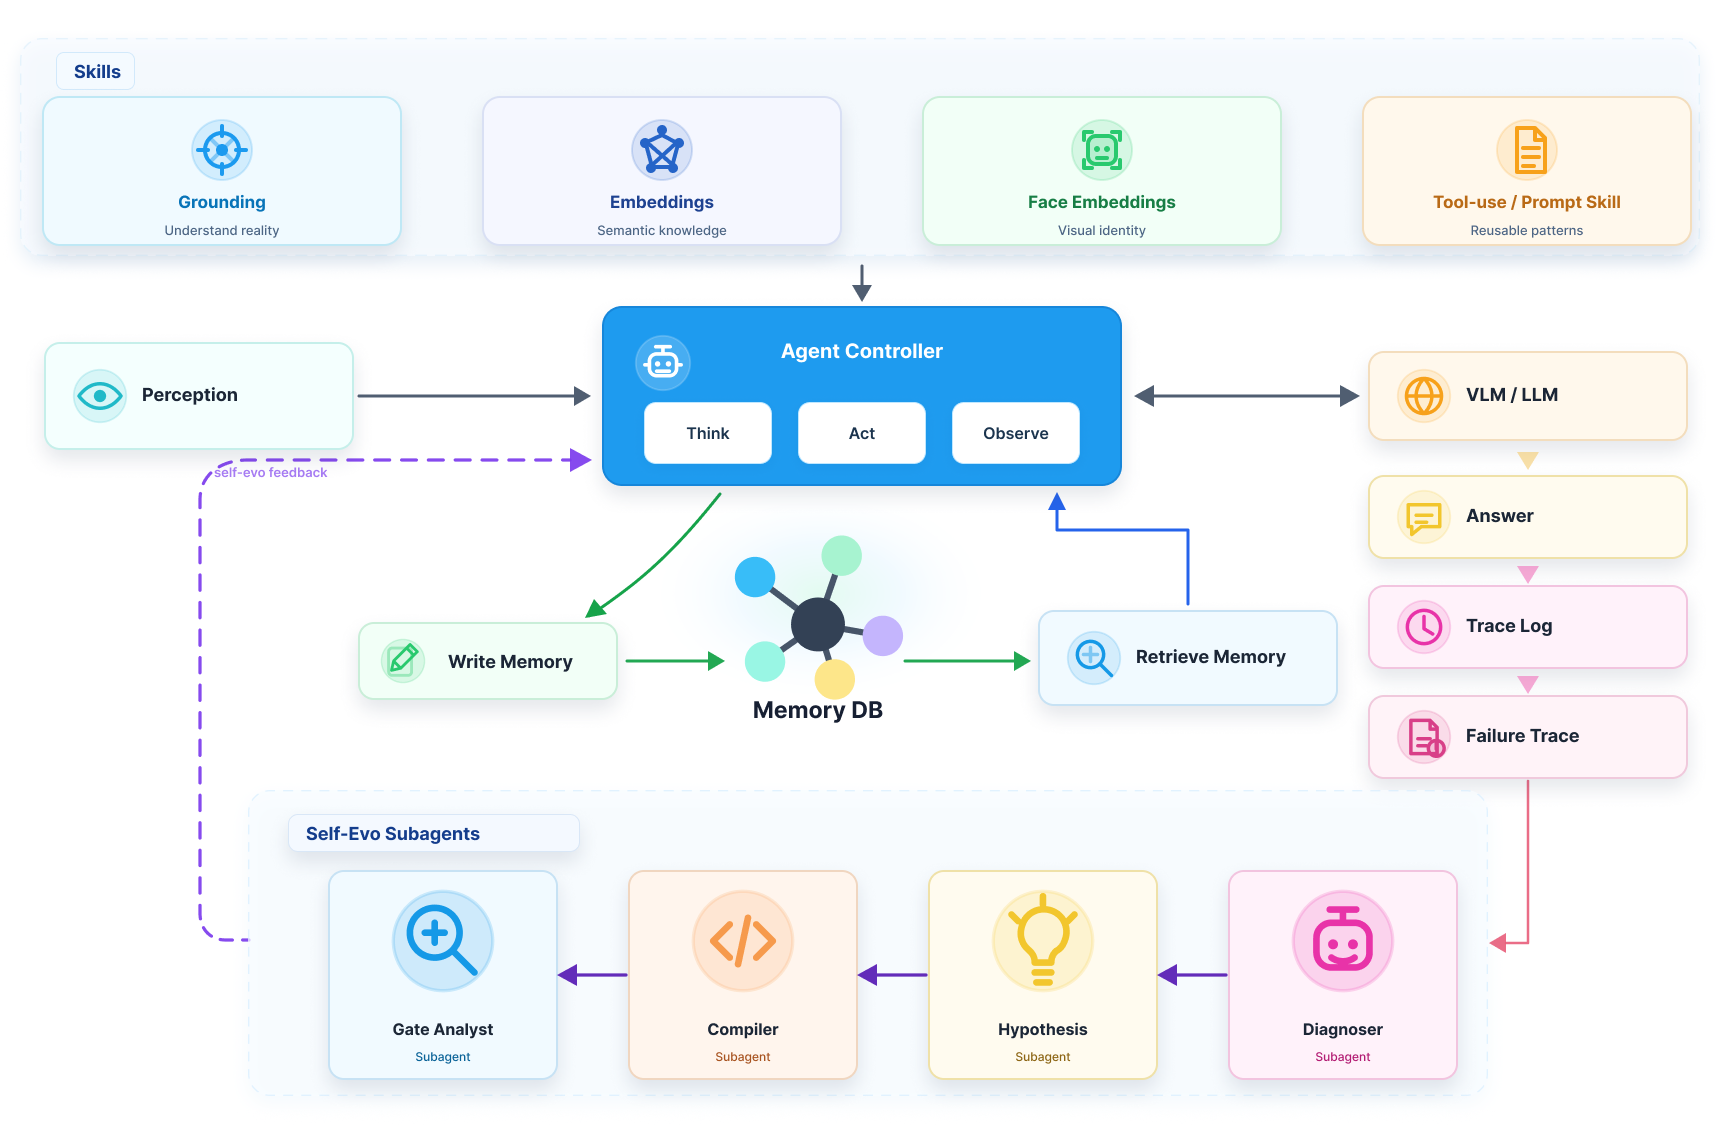
\includegraphics[width=1\linewidth]{figure/architecture2.png}
    \caption{
    Overview of the multi-modal memory architecture.
    During online execution, ABot-AgentOS writes observations and interactions into a source-grounded memory graph, retrieves task-relevant evidence, and records retrieval and answer traces.
    Offline, failure traces are diagnosed and converted into gated runtime evo-assets for later deployments.
    }
    \label{fig:memory_architecture}
\end{figure}

\subsection{Memory System}
\label{sec:memory_system}

Long-horizon embodied interaction requires a memory substrate that is external to the LLM context, persistent across sessions, and grounded in the robot's own experience.
In ABot-AgentOS, the memory system provides this substrate.
It records observations, human--robot dialogue turns, model-extracted semantic facts, visual evidence, identities, object states, spatial relations, and task traces as source-grounded memory records, and makes the accumulated experience available to later reasoning steps through traceable retrieval.
Rather than serving as a raw archive of complete videos, full dialogue transcripts, or unstructured image payloads, the memory system converts multi-modal experience into compact graph records with typed entities, events, relations, temporal context, and provenance.
This design allows the agent to recall people, animals, objects, places, events, temporal facts, spatial relations, and source evidence without overloading the online context window.

The memory system is positioned beneath the online runtime and complements the context management module.
Context management decides what information should be placed in the current prompt, including the current instruction, role strategy, execution plan, recent observations, and reflection summaries.
Memory decides what should persist beyond the current episode and how relevant past evidence should be retrieved back into context.
This separation prevents long-term memory from degenerating into an unstructured prompt dump while still allowing the agent controller to use persistent experience when the current task requires identity recall, temporal grounding, object-location recall, or source-backed visual evidence.

A practical robotic memory must satisfy three requirements. First, it
must be multi-modal, because useful experience is distributed across
language, egocentric vision, object states, spatial layouts, identities,
and task traces. Second, it must be relational, because embodied recall
often depends on who participated in an event, where an object was last
seen, what changed over time, or which frame supports a claim. Third, it
must be auditable and improvable: each answer should expose its evidence
so failures can be attributed to memory writing, evidence selection,
temporal grounding, visual matching, or answer composition.




% ABot-AgentOS implements these requirements through a unified lifelong multi-modal graph memory.
% Our design is related to recent long-term memory systems, but targets a different operating point.
% Conversational memory systems such as Mem0 and SimpleMem focus on extracting, compressing, and retrieving salient information from long interaction histories \cite{mem0,simplemem}.
% multi-modal memory agents such as M3-Agent and WorldMM further show the benefit of maintaining episodic, semantic, and visual memories over long multi-modal streams \cite{m3agent,worldmm}.
% Memory-centric embodied QA systems also show that memory should not be a passive cache, but should interact with exploration, stopping, retrieval, and answering modules during embodied reasoning \cite{memoryeqa}.
% In contrast, ABot-AgentOS focuses on physically grounded robotic memory: the memory must preserve not only textual facts, but also visual evidence, spatial relations, identity continuity, temporal context, source provenance, and task traces in a single auditable graph.

% The memory system persists selected embodied experience across sessions, including human--robot dialogue, visual observations, observed identities, object states, local scene records, semantic events, and task traces.
% These records are organized within a graph substrate that supports both semantic retrieval and relational reasoning.
% Each memory item is stored as a typed node with compact, source-grounded metadata, while typed edges encode temporal order, containment, appearance, identity, location, participation, attachment, spatial relations, and interaction relations.
% This design allows the agent to retrieve relevant past evidence as a local evidence subgraph and inject it into the online reasoning context.
% Since the memory schema encodes platform-agnostic semantic experience rather than hardware-specific control details, the same memory interface can be reused across different robot embodiments, while embodiment-specific sensing and action execution remain handled by the perception and skill layers.

\subsubsection{Graph Memory Representation}
\label{sec:memory_representation}

We represent long-term experience as a typed graph
\begin{equation}
    \mathcal{G} = (\mathcal{V}, \mathcal{E}),
\end{equation}
where each node $v \in \mathcal{V}$ denotes an entity or evidence unit, and each edge $e \in \mathcal{E}$ denotes a temporal, semantic, spatial, identity, interaction, or provenance relation.
Each node stores a compact JSON-style information field containing schema version, dataset or source reference, time reference, evidence summary, confidence, adapter-specific fields, and provenance.
Provenance records the source id, adapter version, extractor model, and related extraction metadata, while temporal information is represented through fields such as \texttt{time\_ref}, \texttt{created\_at}, or adapter-specific fields.
Together these fields allow a memory item to be traced back to the observation, video segment, frame, image, or session from which it was created.

% The canonical node types include \texttt{video}, \texttt{scene}, \texttt{frame}, \texttt{event}, \texttt{person}, \texttt{animal}, \texttt{object}, \texttt{place}, \texttt{session}, and \texttt{image}. Edges
% encode the structure needed for embodied recall: temporal order through
% \texttt{NEXT}, containment through \texttt{CONTAINS} or \texttt{PART\_OF}, observation through
% \texttt{APPEARS\_IN} and \texttt{OBSERVED\_IN}, participation through \texttt{PARTICIPATES},
% location through \texttt{LOCATED\_IN}, identity continuity through \texttt{SAME\_AS} or
% identity timelines, and physical relations such as \texttt{ON}, \texttt{INSIDE},
% \texttt{NEAR}, \texttt{HOLDS}, or \texttt{USES}. The schema is intentionally
% platform-agnostic: it stores semantic experience and evidence rather
% than hardware-specific control details, so the same memory interface can
% be reused across robot embodiments.


% The canonical node types include \texttt{video}, \texttt{scene}, \texttt{frame}, \texttt{event}, \texttt{person}, \texttt{animal}, \texttt{object}, \texttt{place}, \texttt{session}, and \texttt{image}.
% These nodes cover both embodied perception and interaction history.
% For example, a video or source record identifies the originating media and source metadata; a frame node stores a selected visual evidence frame; an event node stores a compact semantic fact, action, or state change; a person or animal node stores scene- or session-level identity evidence, appearance evidence, and links to an identity timeline; an object node stores a canonical name, aliases, attributes, state facts, observations, and last-seen information; and a session node represents a dialogue or multi-modal interaction episode.

% For concreteness, an utterance such as ``I adopted a Maltese dog yesterday'' can be written as a compact event node:
% \begin{quote}
% \small
% \begin{verbatim}
% {
%   "type": "event",
%   "subject": "user",
%   "predicate": "adopted",
%   "object": "Maltese dog",
%   "relative_time": "yesterday",
%   "time_ref": "2024-05-22",
%   "evidence": "The user said they adopted a Maltese dog yesterday.",
%   "source_ref": "session_021/turn_003",
%   "confidence": 0.86,
%   "provenance": {
%     "extractor": "writer_model",
%     "schema": "abot_memory_v1"
%   }
% }
% \end{verbatim}
% \end{quote}
% The node is not merely a text chunk: it exposes subject, predicate, object, time, evidence, confidence, source reference, and provenance fields that can later be used for temporal grounding, entity retrieval, and trace inspection.

% Edges encode the structure required for long-horizon reasoning.
% Temporal edges such as \texttt{NEXT} connect scenes, sessions, or identity tracks, with \texttt{info.next\_kind} distinguishing scene timelines, session timelines, person identity timelines, and animal identity timelines.
% Containment edges such as \texttt{CONTAINS} connect scenes or sessions to event nodes, while \texttt{PART\_OF} connects selected frame nodes to their parent scenes.
% Observation edges such as \texttt{APPEARS\_IN} associate people, animals, or objects with scenes, while \texttt{OBSERVED\_IN} attaches object observations to selected evidence frames.
% Participation edges such as \texttt{PARTICIPATES} connect people, animals, and objects to the semantic events in which they take part.
% Grounding edges such as \texttt{LOCATED\_IN} attach events and objects to places.
% Identity continuity is represented primarily by typed \texttt{NEXT} identity timelines across scene-level person or animal nodes, while \texttt{SAME\_AS} can be used for cross-frame or cross-source equivalence links.
% Spatial edges such as \texttt{ON}, \texttt{UNDER}, \texttt{INSIDE}, \texttt{NEAR}, \texttt{LEFT\_OF}, \texttt{RIGHT\_OF}, \texttt{IN\_FRONT\_OF}, and \texttt{BEHIND} encode physically meaningful object-object relations.
% Interaction edges such as \texttt{HOLDS}, \texttt{TOUCHES}, \texttt{USES}, \texttt{GIVES\_TO}, and \texttt{LOOKS\_AT} encode person/object or animal/object interactions.
% Image attachment edges such as \texttt{ATTACHED\_TO} connect multi-modal evidence to the semantic events it supports.

% \begin{table}[!t]
%     \centering
%     \small
%     \begin{tabular}{p{0.20\linewidth}p{0.72\linewidth}}
%         \toprule
%         \textbf{Memory element} & \textbf{Role in embodied recall} \\
%         \midrule
%         Entity nodes &
%         Represent persistent entities and evidence units, including people, animals, objects, places, sessions, images, selected frames, and semantic events. \\

%         Temporal edges &
%         Preserve scene order, session order, and identity timelines for questions involving before/after relations or relative dates. \\

%         Identity timelines &
%         Bind scene-level person or animal evidence across time using typed \texttt{NEXT} edges, with optional \texttt{SAME\_AS} links for cross-source equivalence. \\

%         Spatial and interaction edges &
%         Encode physical relations such as \texttt{ON}, \texttt{UNDER}, \texttt{INSIDE}, and \texttt{NEAR}, as well as interactions such as \texttt{HOLDS}, enabling spatially and action-grounded recall. \\

%         Provenance fields &
%         Preserve source references and extractor metadata so that answers can be audited against the retrieved evidence. \\
%         \bottomrule
%     \end{tabular}
%     \caption{Key components of the ABot-AgentOS memory graph.}
%     \label{tab:memory_graph_components}
% \end{table}

% This graph formulation is motivated by recent spatial and embodied memory systems.
% SpatialMem builds a queryable memory that unifies 3D geometry, semantics, and language with metric anchors and open-vocabulary object nodes \cite{spatialmem}.
% 3DLLM-Mem studies long-term spatial-temporal memory for embodied 3D LLMs, where working-memory tokens selectively attend to episodic spatial and temporal features \cite{threedllmmem}.
% DAAAM constructs hierarchical 4D scene graphs as real-time spatio-temporal memory for large-scale embodied question answering \cite{daaam}.
% Compared with these systems, our graph representation is less tied to a single 3D reconstruction pipeline and instead provides a general memory schema for dialogue, visual evidence, identities, places, events, temporal relations, provenance, and robot task traces.


The schema includes nodes for source containers, evidence units, entities, places, sessions, and semantic events.
Edges encode the relations needed for embodied recall, including temporal order, containment, observation, participation, location, identity continuity, spatial relations, and interaction relations.
The schema is intentionally platform-agnostic: it stores semantic experience and evidence rather than hardware-specific control details, so the same memory interface can be reused across robot embodiments.

This representation differs from conventional retrieval-augmented generation over text chunks.
Text retrieval mainly returns semantically similar snippets, whereas the memory graph first identifies relevant seed nodes and then expands to a local evidence subgraph for reasoning over identity, time, location, participation, provenance, and spatial relations.
As a result, the agent can answer questions about object locations, identity continuity, or relative time using structured evidence rather than parametric memory alone.

\subsubsection{Multi-modal Memory Updating}
\label{sec:memory_writing}


Memory updating can occur during interaction and at reflection checkpoints.
In an online ABot-AgentOS deployment, the controller receives observations, tool results, dialogue turns, and execution traces, while a memory-writing service selects information from these streams and converts it into compact graph records linked to session, place, time, source reference, and provenance.
We instantiate this writer as a set of graph-construction adapters for different data sources and applications.
This design does not modify the robot action space; instead, it augments the agent's reasoning state with persistent, source-grounded evidence that can be retrieved in later tasks.


% For video observations, and for egocentric streams when they are represented as video-like episodes, the default writing pipeline first performs global person and animal detection, then applies VLM-based scene and frame understanding to extract visible entities, object states, place descriptions, actions, and semantic events.
% The system creates scene, frame, event, person, animal, object, and place nodes, while the video/source container is represented through source metadata such as \texttt{source\_id} and \texttt{source\_ref}.
% It then adds timeline, containment, observation, participation, location, identity-timeline, and spatial or interaction edges.
% Selected frames are stored as evidence nodes and source references rather than as the only memory representation; the primary memory item is a compact semantic or entity record linked back to its source.

% For dialogue and multi-modal sessions, dataset or application adapters create session nodes and compact semantic event nodes, with optional image nodes for multi-modal attachments.
% The writer favors semantic compression over raw full-turn storage, following the principle that long-term memory should increase information density rather than preserve raw histories verbatim.
% Recent work such as SimpleMem further shows that structured semantic compression and query-aware retrieval can improve memory efficiency under limited context budgets~\cite{simplemem}.
% In ABot-AgentOS, this principle is instantiated through graph writing: raw observations are converted into typed, source-grounded nodes and edges that can later be queried by content, time, entity mention, modality, provenance, and relation.

To support abstraction across modalities, different inputs are normalized into the same source-grounded graph schema.
Video and egocentric streams produce semantic records for visible entities, object states, places, actions, frames, and events; dialogue and multi-modal sessions produce session-level and event-level records, with image attachments stored as evidence nodes connected to the corresponding semantic event.
Across these inputs, the writer favors semantic compression over raw full-turn or full-frame storage, following the principle that long-term memory should increase information density without sacrificing traceability.
Recent work such as SimpleMem further shows that structured semantic compression and query-aware retrieval can improve memory efficiency under limited context budgets~\cite{simplemem}.
In ABot-AgentOS, this principle is instantiated by converting raw observations into typed, source-grounded nodes and edges that can later be queried by content, time, entity mention, modality, provenance, and relation.
For instance, the utterance ``I adopted a Maltese dog yesterday'' is represented as a time-grounded semantic event that links the utterance, resolved temporal context, identity hypothesis, confidence estimate, and source evidence, rather than as a raw transcript line.
When an image is attached, the image node is connected to the event as supporting multi-modal evidence.
This conversion allows multi-modal observations to support temporal grounding, identity resolution, provenance-aware retrieval, and graph-based reasoning.
Concrete examples of how such records support retrieval and later failure-driven improvement are shown in Figure~\ref{fig:mem_example}.

The same principle also governs what is written and how the graph is maintained over time.
Not every raw observation becomes a permanent memory item: the writer prioritizes information likely to support future embodied or interaction tasks, including identities, object locations, state changes, social commitments, user preferences, abnormal events, temporal facts, and evidence needed for later verification.
After insertion, ABot-AgentOS performs lightweight maintenance to keep the graph compact over long horizons.
Near-duplicate entity or event nodes are merged when they share compatible provenance, temporal context, and identity evidence; frequently observed entities keep compact state summaries with a bounded set of representative evidence nodes.
Stale state facts are superseded by newer observations through temporal edges rather than deleted immediately, allowing retrieval to distinguish current state from historical evidence.
Together, selective writing and post-insertion maintenance reduce storage cost, avoid redundant low-level records, and preserve enough source-grounded evidence for later auditability.



% Different modalities are normalized into the same source-grounded graph schema.
% Video and egocentric streams produce semantic records for visible entities, object states, places, actions, frames, and events; dialogue and multi-modal sessions produce session-level and event-level records, with image attachments stored as evidence nodes connected to the corresponding semantic event.
% Across these inputs, the writer favors semantic compression over raw full-turn or full-frame storage, following the principle that long-term memory should increase information density without sacrificing traceability.
% Recent work such as SimpleMem further shows that structured semantic compression and query-aware retrieval can improve memory efficiency under limited context budgets~\cite{simplemem}.
% In ABot-AgentOS, this principle is instantiated by converting raw observations into typed, source-grounded nodes and edges that can later be queried by content, time, entity mention, modality, provenance, and relation.

% For instance, the utterance ``I adopted a Maltese dog yesterday'' is not stored merely as a raw text line.
% Instead, it is converted into a time-grounded semantic event containing subject, predicate, object, evidence, relative time, resolved time, session reference, confidence, and provenance fields.
% When entity resolution or temporal normalization is available, the record can also be linked to an animal identity hypothesis and to the resolved date.
% Similarly, an image attachment can become an \texttt{image} node connected to the supporting semantic event through \texttt{ATTACHED\_TO}, with image identifiers, captions, source references, and embeddings supporting later retrieval.
% This conversion transforms multi-modal observations into structured evidence that supports temporal grounding, identity resolution, provenance-aware retrieval, and graph-based reasoning.
% Concrete examples of how such records support retrieval and later failure-driven improvement are shown in Figure~\ref{fig:mem_example}.

% For instance, the utterance ``I adopted a Maltese dog yesterday'' is represented as a time-grounded semantic event that links the utterance, resolved temporal context, identity hypothesis, confidence estimate, and source evidence, rather than as a raw transcript line.
% When an image is attached, the image node is connected to the event as supporting multi-modal evidence.
% This conversion allows multi-modal observations to support temporal grounding, identity resolution, provenance-aware retrieval, and graph-based reasoning.
% Concrete examples of how such records support retrieval and later failure-driven improvement are shown in Figure~\ref{fig:mem_example}.

% Memory writing is selective.
% Not every raw observation becomes a permanent memory item; the writer prioritizes information likely to support future embodied or interaction tasks, including identities, object locations, state changes, social commitments, user preferences, abnormal events, temporal facts, and evidence needed for later verification.
% This reduces storage cost and avoids filling the database with redundant low-level observations, while source references, temporal context, evidence summaries, and provenance fields preserve the information needed for auditability.

% \paragraph{Memory Maintenance.}
% To keep the graph compact over long horizons, ABot-AgentOS performs lightweight maintenance after insertion.
% Near-duplicate entity or event nodes are merged when they share compatible provenance, temporal context, and identity evidence; frequently observed entities keep compact state summaries with a bounded set of representative evidence nodes.
% Stale state facts are superseded by newer observations through temporal edges rather than deleted immediately, allowing retrieval to distinguish current state from historical evidence.
% This policy preserves auditability while preventing the graph from growing into a raw observation dump.

\subsubsection{Retrieval and Grounded Answering}
\label{sec:memory_retrieval}

At runtime, memory retrieval is invoked when the current task requires information beyond the immediate observation or short-term context.
The query is converted into semantic retrieval signals and, when available, lightweight structural cues such as entity mentions, temporal expressions, modality, place references, and expected evidence type.
The retriever first selects candidate seed nodes using semantic embeddings, lexical matching, metadata filters, source constraints, and node-type constraints.
Given a query $q$, this hybrid seed selection can be written as
\begin{equation}
    s(q,v) =
    \lambda_{\mathrm{sem}} s_{\mathrm{sem}}(q,v)
    + \lambda_{\mathrm{lex}} s_{\mathrm{lex}}(q,v)
    + \lambda_{\mathrm{meta}} s_{\mathrm{meta}}(q,v)
    + \lambda_{\mathrm{type}} s_{\mathrm{type}}(q,v),
    \label{eq:hybrid_retrieval_score}
\end{equation}
where $s_{\mathrm{sem}}$ denotes embedding similarity, $s_{\mathrm{lex}}$ denotes lexical overlap, $s_{\mathrm{meta}}$ measures metadata compatibility such as time, source, modality, or place, and $s_{\mathrm{type}}$ favors node types expected by the query.
The top-ranked seeds are then expanded along task-relevant typed edges under a fixed depth and evidence-token budget, producing a local evidence subgraph that contains the semantic, temporal, spatial, identity, and provenance context needed for answering.
This differs from retrieval over independent memory stores, as in dynamic multi-modal retrieval agents such as WorldMM~\cite{worldmm}: ABot-AgentOS retrieves seed nodes and then expands a typed graph neighborhood, so the answerer can reason over relations among evidence items rather than over isolated snippets.
The resulting subgraph is serialized as a compact evidence context, paired with a retrieval trace, and injected into the agent's reasoning context.

% This retrieval process is complementary to dynamic multi-modal retrieval agents such as WorldMM, which adaptively selects among episodic, semantic, and visual memories at different temporal granularities for long-video reasoning \cite{worldmm}.
% Instead of selecting among separate memory stores, ABot-AgentOS performs query-dependent seed retrieval followed by typed graph expansion, allowing the answerer to reason over a local evidence subgraph containing semantic, temporal, spatial, identity, and provenance evidence.

The answerer is instructed to ground its response in retrieved evidence.
This is particularly important for embodied and interaction-memory questions, where the correct answer often depends on local experience, temporal grounding, or visual evidence rather than general world knowledge.
When evidence is insufficient or contradictory, the answerer is expected to report uncertainty instead of hallucinating an unsupported fact; in forced-choice benchmark settings, it still records the evidence limitation in the trace.

Each memory-augmented QA run records a retrieval trace containing the retrieved nodes and edges, source references, evidence summaries, retrieval stages, and ranking signals.
In online deployment, this trace makes the answer inspectable and can help the controller decide whether additional observation or clarification is required.
Offline, it provides the diagnostic signal for failure analysis: an incorrect answer can be attributed to missing memory writing, failed retrieval, evidence misuse, or unresolved temporal, spatial, relation-direction, or entity-grounding operations.

\begin{figure}[!t]
    \centering
    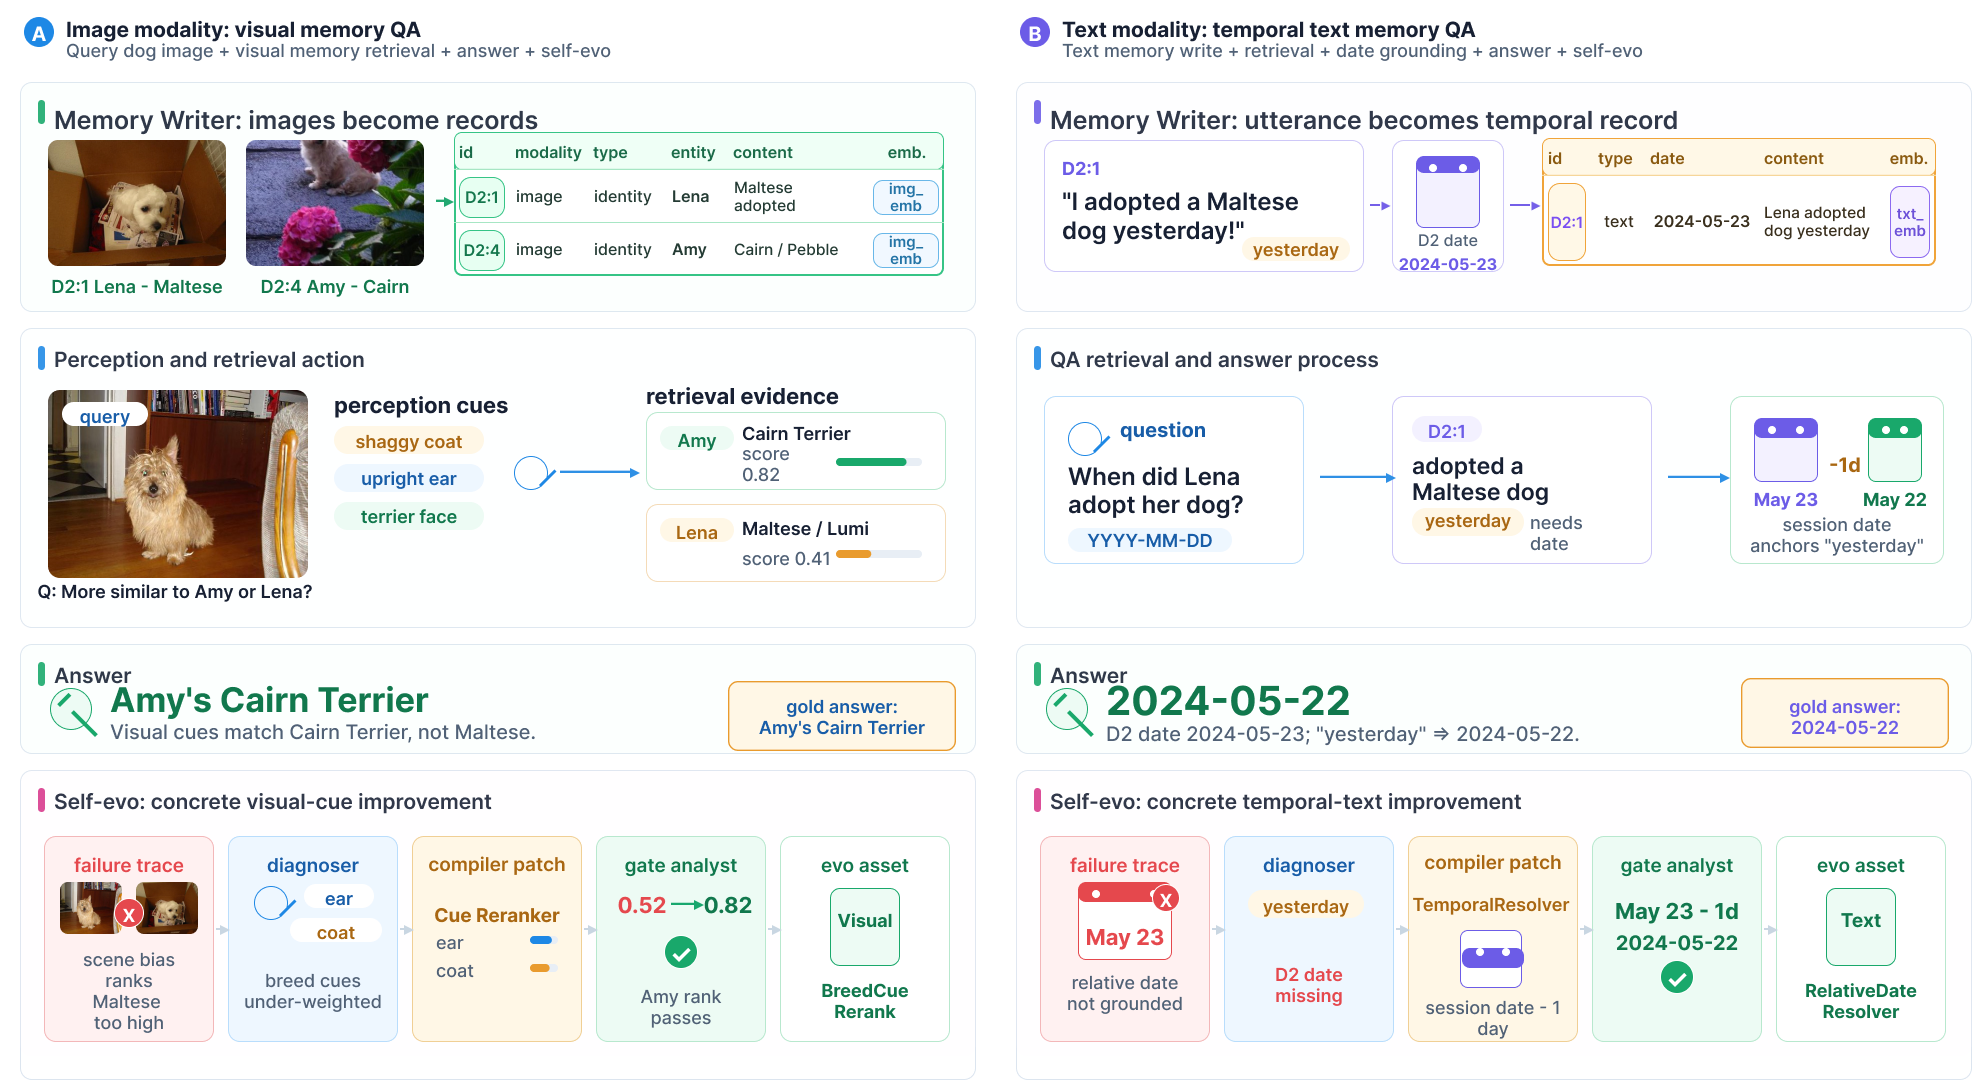
\includegraphics[width=1\linewidth]{figure/mem_example.png}
    \caption{
    Concrete memory failure-to-evolution examples.
    Left: visual memory QA retrieves image-grounded identity evidence but can expose missing breed-specific cues.
    Right: temporal text memory QA uses session metadata to resolve relative dates but can reveal temporal-normalization errors.
    In both cases, the failure trace is converted into targeted memory-writing, evidence-selection, frame-selection, or answering improvements.
    }
    \label{fig:mem_example}
\end{figure}

\subsubsection{Failure-Driven Lifelong Self-Evolution}
\label{subsubsec:memory-self-evolution}

% Recent work on self-evolving agents argues that deployed agent systems should not remain static, but should improve their components from interaction data, environmental feedback, and test-time trajectories \cite{selfevolvingsurvey}.
% This view is particularly important for long-term memory: if only the stored contents are updated while the writer, evidence-selection policy, and answerer remain fixed, the memory system can repeatedly make the same extraction, retrieval, grounding, or reasoning mistakes.
% Evo-Memory formulates this issue as a streaming test-time learning problem, where agents must continuously retrieve, integrate, update, and reuse memory across evolving task sequences \cite{evomemory}.
% Recent self-evolving memory systems further show that memory evolution can target different levels of the pipeline, including retrieval configurations, memory architectures, procedural memories, memory skills, and multi-agent memory-cycle coordination \cite{evolvemem,memevolve,reme,memskill,memma}.
% In addition, evidence-gap-driven and evidence-verifiable self-evolution highlights the need to diagnose missing evidence and only learn from source-grounded, auditable signals \cite{evimem,eveagent}.

Long-term memory should evolve not only by accumulating new content, but also by improving the pipeline that writes, retrieves, selects, and uses evidence.
Otherwise, the system may repeatedly make the same extraction, retrieval, temporal-grounding, visual-selection, or answer-composition errors even as the memory graph grows.
This view is aligned with recent work on self-evolving agents, streaming memory evolution, and evidence-verifiable improvement, which emphasizes learning from interaction traces while keeping updates auditable and bounded \cite{selfevolvingsurvey,evomemory,evolvemem,memevolve,reme,memskill,memma,evimem,eveagent}.



Figure~\ref{fig:memory_architecture} shows the online memory components and the offline self-evolution loop at a system level, while Figure~\ref{fig:mem_example} gives concrete examples of how memory failures become targeted evo-assets.
We formalize this process as a split-wise protocol over long-term deployment, or its benchmark approximation, represented by an ordered sequence of disjoint splits
$\mathcal{D}_1,\ldots,\mathcal{D}_T$.
At split $t$, ABot-AgentOS maintains two persistent states: the accumulated memory graph $G_{t-1}$ and the promoted evo-asset set $A_{<t}$.
The graph stores content-level experience, including entities, events, places, visual evidence, temporal context, and provenance, while evo-assets store pipeline-level improvements for memory writing, evidence selection, graph expansion, answer composition, frame selection, temporal normalization, or adapter-level normalization.
During online execution, the agent writes new observations into memory, retrieves evidence for downstream answering, and records retrieval and answer traces under the currently promoted asset set.
Only after split $t$ has been evaluated are failed cases converted into failure traces and processed for possible improvement.
No evo-asset generated from split $t$ is used during inference on split $t$; accepted assets are promoted only for later splits.
This no-leakage constraint turns self-evolution into a cumulative lifelong process rather than a one-shot post-hoc repair.

% Figure~\ref{fig:memory_architecture} shows the online memory components and the offline self-evolution loop at a system level, while Figure~\ref{fig:mem_example} gives concrete examples of how memory failures become targeted evo-assets.
% We formalize the split-wise protocol here without introducing an additional figure.
% We view long-term deployment, or its benchmark approximation, as an ordered sequence of disjoint splits
% $\mathcal{D}_1,\ldots,\mathcal{D}_T$.
% At split $t$, the online memory system maintains two persistent states: the accumulated memory graph $G_{t-1}$ and the promoted evo-asset set $A_{<t}$.
% The memory graph stores content-level experience, including entities, events, places, sessions, visual evidence, temporal context, and provenance.
% The evo-assets store pipeline-level improvements, including writer rules, retrieval-side policies for query normalization, evidence filtering, edge-expansion priority, and evidence serialization within the fixed hybrid retrieval architecture, answerer instructions, frame-selection policies, temporal-normalization policies, and dataset- or application-specific normalization rules.

% During online execution, the agent writes new observations into memory, retrieves evidence for downstream answering, and records retrieval and answer traces.
% After split $t$ has been evaluated, failed cases are converted into failure traces and processed by the offline self-evolution loop.
In benchmark settings, failures are identified using ground-truth answers only after the split is complete; in deployment, analogous feedback can come from environmental signals, task success or failure, human correction, or low-confidence retrieval and answering traces.
Only assets that pass the gate are promoted and used in later splits.
No evo-asset generated from split $t$ is used during inference on split $t$.
This split-wise protocol prevents evo-assets from using supervision from the same split on which they are evaluated, turning self-evolution into a cumulative lifelong process rather than a one-shot post-hoc repair.

Formally, the online run, asset proposal, and asset promotion steps are:
\begin{align}
    \mathcal{T}_t, G_t
    &= \operatorname{Run}(\mathcal{D}_t; G_{t-1}, A_{<t}), \\
    \Delta A_t
    &= \operatorname{Gate}\!\left(
        \operatorname{Compile}\!\left(
        \operatorname{Propose}\!\left(
        \operatorname{Diagnose}(\mathcal{T}_t)
        \right)\right)\right), \\
    A_{\leq t}
    &= A_{<t} \cup \Delta A_t .
    \label{eq:self_evo_update}
\end{align}
Here $\mathcal{T}_t$ denotes the answer traces and failure traces collected on split $t$.
Only $A_{\leq t}$ is available for later splits $\mathcal{D}_{t+1},\ldots,\mathcal{D}_T$.

% Within each split, ABot-AgentOS runs the normal online memory pipeline without changing the base model or the active asset set.
% After the split, the collected traces are used by an offline multi-agent self-evolution loop.
% When supervision is available, a failed QA attempt is converted into a failure trace containing the question, retrieved evidence, prediction, expected answer, retrieval trace, and dataset context.
% A Diagnoser analyzes the failure source, distinguishing among memory-writing errors, evidence-selection misses or ranking errors, answer-composition errors, frame-selection errors, temporal-normalization errors, entity or subject mismatches, relation-direction errors, and adapter-specific errors.
% A Hypothesis Generator proposes candidate fixes.
% A Compiler-Critic converts safe fixes into a constrained JSON DSL asset.

After each split, the collected traces are processed by a constrained failure-to-asset loop.
When supervision is available, a failed QA attempt is represented by the question, retrieved evidence, prediction, expected answer, retrieval trace, and dataset context; in deployment, analogous feedback can come from environmental signals, task outcomes, human correction, or low-confidence traces.
The loop diagnoses the failure source, proposes a candidate repair, compiles the repair into a constrained JSON DSL evo-asset, and evaluates it with both target and regression checks.
This follows the broader principle of safe resource evolution: prompts, tools, memory modules, and other agent resources should be versioned, auditable, and rollbackable rather than updated through unconstrained code generation \cite{autogenesis}.


% Finally, a Gate Analyst evaluates the candidate on the target and regression splits and accepts it only if it improves target behavior without introducing unacceptable regressions.
% This design follows the broader principle of safe resource evolution: prompts, tools, memory modules, and other agent resources should be versioned, auditable, and rollbackable rather than updated through unconstrained code generation \cite{autogenesis}.

% \begin{table}[!t]
%     \centering
%     \small
%     \begin{tabular}{p{0.20\linewidth}p{0.33\linewidth}p{0.35\linewidth}}
%         \toprule
%         \textbf{Agent} & \textbf{Input} & \textbf{Output} \\
%         \midrule
%         Diagnoser &
%         Failure trace, retrieved evidence, expected answer, dataset context &
%         Failure type and root-cause explanation. \\

%         Hypothesis Generator &
%         Diagnosis and memory-pipeline context &
%         Candidate repair hypothesis targeting writer, evidence selection, answerer, frame policy, or adapter behavior. \\

%         Compiler-Critic &
%         Candidate hypothesis and safety constraints &
%         Constrained JSON DSL evo-asset with no generated Python execution. \\

%         Gate Analyst &
%         Candidate asset, target subset, regression subset &
%         Accept/reject decision, validation report, and regression report. \\
%         \bottomrule
%     \end{tabular}
%     \caption{Roles in the offline self-evolution loop.}
%     \label{tab:self_evo_agents}
% \end{table}

The gate evaluates each candidate asset on a target validation subset and a regression subset.
An asset $a$ is accepted only if it improves the target score by at least $\tau_{\mathrm{gain}}$ and does not reduce the regression score by more than $\tau_{\mathrm{reg}}$:
\begin{equation}
    \operatorname{Accept}(a)=
    \mathbb{I}\left[
    \Delta S_{\mathrm{target}}(a) \geq \tau_{\mathrm{gain}}
    \land
    \Delta S_{\mathrm{reg}}(a) \geq -\tau_{\mathrm{reg}}
    \right].
    \label{eq:gate_criterion}
\end{equation}
This criterion makes promotion conservative: an asset must improve the failure pattern it targets while preserving behavior on previously reliable cases.

Accepted evo-assets are lifecycle-managed JSON DSL records and do not execute generated Python code.
Each asset declares its target layer, triggering condition, permitted action, safety constraints, provenance, validation result, and version id.
Assets may target memory writing, evidence selection, answer composition, visual frame selection, temporal normalization, or adapter-level normalization.
Normal QA behavior is unchanged unless accepted assets are explicitly loaded; writer-side and frame-policy assets require fresh graph construction, whereas evidence-selection and answerer assets can be loaded at runtime.
In this way, ABot-AgentOS accumulates two forms of lifelong knowledge: content-level experience in the memory graph and pipeline-level improvements in the evo-asset set.


% Evo-assets can target different layers of the memory pipeline.
% Writer assets improve fact extraction, entity normalization, temporal grounding, and graph construction.
% Evidence-selection assets adjust query normalization, seed-node ranking, edge-expansion priorities, evidence filtering, or evidence serialization inside the base hybrid graph retriever.
% Answerer assets improve the use, calibration, and formatting of retrieved evidence.
% Frame-policy assets improve the selection of visual evidence frames.
% Data-adapter assets are represented in the DSL but used conservatively when dataset-specific normalization is required.
% Normal QA behavior is unchanged unless accepted assets are explicitly loaded.
% Writer-side and frame-policy assets require fresh graph construction so that improvements to memory writing or visual evidence selection are reflected in the stored graph, whereas evidence-selection and answerer assets can be loaded at runtime.

% This failure-driven process turns memory errors into reusable system improvements.
% For example, if a visual memory QA failure shows that breed-specific cues such as ear shape or coat texture were underweighted, the self-evolution loop can propose an evidence-selection, answerer, or frame-policy asset that emphasizes those cues in evidence selection or answer composition.
% If a temporal text QA failure shows that the model treated ``yesterday'' as the session date instead of session date minus one day, the loop can propose a writer, temporal-normalization, or answerer policy asset that improves the use of temporal metadata.
% The gate prevents such candidate assets from being promoted unless they improve later held-out behavior without unacceptable regressions.
% In this way, the system accumulates two forms of lifelong knowledge: content-level experience in the memory graph and pipeline-level improvements in the evo-asset set.

\subsubsection{Edge-Cloud Collaborative Memory Management}
\label{sec:memory-sync}

Embodied agents continuously acquire heterogeneous memories during interaction with the physical world, including maps, semantic landmarks, obstacles, objects, and human-related observations. 
While public environmental memories, such as roadblocks, construction areas, and navigational landmarks, can improve multi-agent collaboration when shared, privacy-sensitive memories, such as faces, personal belongings, or person-associated objects, must remain local. 
To address this conflict, we design an edge-cloud collaborative memory system that separates private memory on the robot from common memory in the cloud.

\paragraph{Memory Partition}
Each robot maintains a private memory at the edge, which stores all locally perceived memories, including map memory, semantic memory, and multi-modal memory. 
The cloud maintains a common memory that only contains public, low-sensitivity memories useful for collective navigation and task execution. 
This design follows a private-by-default principle: a memory item is never uploaded unless it is explicitly classified as shareable.

\paragraph{Privacy-aware Memory Gating}
For each newly generated memory item, the system performs a privacy judgment before synchronization. 
A memory is regarded as non-shareable if it contains or is associated with personally identifiable information, including persons, faces, names, personal objects, or ownership relations to a specific individual. 
In contrast, public environmental information, such as maps, traffic cones, barriers, road damage, and static landmarks, is classified as shareable.


To evaluate the reliability of the privacy protection mechanism, we constructed a dedicated dataset for privacy classification and upload-decision testing. Experimental results show that the system achieves over 99\% accuracy in identifying whether a memory item is suitable for cloud synchronization. This high-accuracy privacy judgment significantly reduces the risk of uploading sensitive user or environment-specific information, while still allowing non-sensitive public knowledge to be shared across robots. As a result, the proposed memory system balances two key requirements of embodied intelligence: preserving user privacy through edge-side private memory, and enhancing group-level collaboration through cloud-side common memory.



% \subsubsection{Summary}
% \label{sec:memory_summary}

% The memory system provides three advantages for a general robotic AgentOS.
% First, it supports cross-modal binding: entities and evidence records can be linked to dialogue mentions, visual appearances, embeddings, locations, temporal events, image attachments, and source evidence.
% Second, it supports relational recall: the agent can answer questions that require following edges across time, space, identity timelines, participation, provenance, and spatial relations rather than retrieving isolated text chunks.
% Third, it supports lifelong improvement: because each memory-augmented QA run is associated with a retrieval trace, failures can be attributed to specific stages of the memory pipeline and converted into gated runtime assets.
% The split-wise lifelong protocol carries accepted evo-assets from earlier splits to later splits, so ABot-AgentOS accumulates both embodied experience in the memory graph and reusable pipeline improvements in the asset set.
% Thus, memory becomes not only a persistent record of embodied and interaction experience, but also the substrate through which ABot-AgentOS improves across long interaction horizons.
% The memory graph accumulates what the robot has experienced, while the evo-asset set improves how that experience is written, selected, grounded, and used.

